\documentclass[11pt,twocolumn]{article}
\usepackage{amsmath}
\usepackage[margin=1in]{geometry}
\usepackage{graphicx}
\usepackage{import}
\usepackage{subfig}

\title{Vision-Based Autonomous Ground Vehicle Navigation}
\date{March 31, 2011}
\author{
	Michael Koval \\
	mkoval@eden.rutgers.edu \\
	Electrical and Computer Engineering
}

\begin{document}
\maketitle

\section{Introduction}
\label{sec:intro}
% 1. Overall description of IGVC
The Intelligent Ground Vehicle Competition (IGVC) is an international collegiate
robotics competition that tasks teams of undergraduate students to design,
build, and program a fully autonomous mobile ground vehicle. Specifically, the
competition consists of three distinct challenges: navigating through a winding
obstacle course, travelling between global positioning system (GPS) waypoints in
large field, and responding to messages broadcast by a Joint Architecture for
Unmanned Systems (JAUS) control system. In each of these tasks, the team has no
knowledge of the course prior to competing and navigation is further complicated
by the addition of road obstacles such as cones, barriers, switchbacks, and
potholes in the drivable regions of the course.

% 2. Alternatives to vision used by other teams
% 3. Importance of vision
Remaining in the course while autonomously navigating around these obstacles
requires that the robot has accurate knowledge of its location and objects in
its surrounding environment. Previous competitors have successfully detected
road obstacles using a combination of scanning laser range finders (LIDAR) and
stereo reconstruction. Unlike LIDAR, stereo reconstruction is capable of
providing three-dimensional data for all points in a scene, instead of only
those that are coplanar with the scanning laser rangefinder. In addition to
using stereo vision to detetct obstacles, image processing is necessary to
identify the course's painted boundaries and to locate the flags that are used
to indicate areas of safe travel.

% 4. Primary vision tasks
With the importance of computer vision clearly understood, the remainder of this
paper will discuss specific algorithms designed for use on the Navigator,
Rutgers Univeristy's entry into the 2011 Intelligent Ground Vehicle Competition.
Before discussing specific computer vision algorithms Section ~\ref{sec:robot}
describes the mechanical, sensing, and computing capabilities of the Navigator
at a high level. Making use of the onboard cameras, Section ~\ref{sec:stereo}
describes the Navigator's baseline-multiplexing stereo vision system and Section
~\ref{sec:lane} discusses monocular tracking of boundary lines. Object
recognition, such as the detection of flags and potholes, is outside the scope
of this paper and is briefly discussed as future work.

\section{Economics}
\label{sec:econ}
% ???

\section{Rutgers Navigator}
\label{sec:robot}
% 1. Brief discussion of mechanical design
% FIGURE: CAD Model and Actual Robot

\begin{figure}
	\centering
	% TODO: Replace this with an actual photo.
	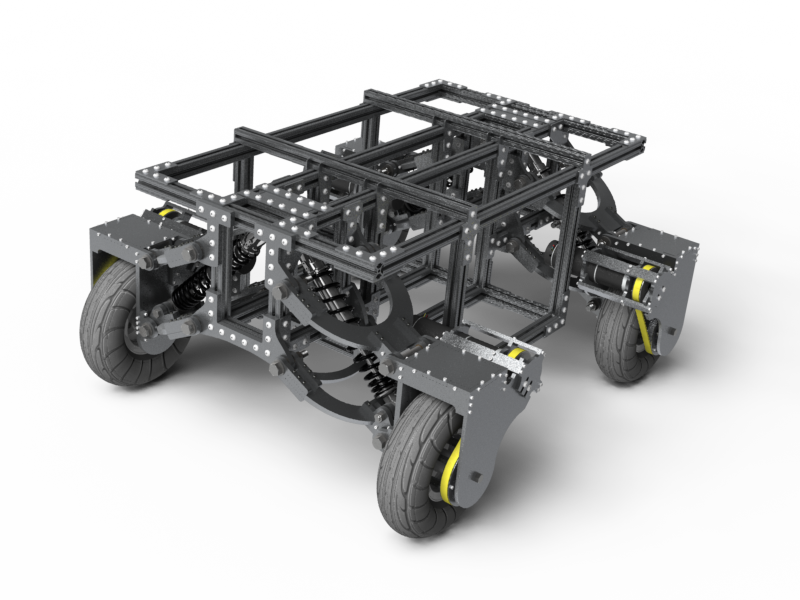
\includegraphics[width=\columnwidth]{include/navigator-cad}
	\caption{CAD render of the Navigator.}
	\label{fig:robot-cad}
\end{figure}

% 2. Sensing capabilities
% 3. Computing capabililities and software architecture
% 4. Integration of vision with path planning (i.e. costmaps)

\section{Stereo Reconstruction}
\label{sec:stereo}
% 1. Selection of the PS3 Eye camera
Stereo vision on a mobile robot is a non-trivial problem that has traditionally
required costly hardware that support high frame rates and hardware
synchornization, such as the Bumblebee stereo vision camera. Thankfully, the
inexpensive Playstation Eye camera uses the OmniVision OV7720 capable of frame
rates up to 125 Hz and can be easily modified to support hardware
synchronization. Mounted in a custom polycarbinate case, three of these cameras
are used for stereo reconstruction.

% 2. Hardware and software camera synchronization
% FIGURE: Justification for synchronization
% FIGURE: Synchronized and desynchronized osilloscope output
% FIGURE: Synchronized and desynchronized images of a clock
\subsection{Synchronization}
\label{sec:stereo-sync}
Even if the cameras used for stereo reconstruction are attached to the same
computer and set to the same frame rate, there is no guarantee that frames will
be captured simultaeously from both cameras. If the cameras are in motion (such
as being attached to a moving robot) this delay changes the effective baseline
of the stereo system and invalidates the camera calibration\footnote{Assuming a
framerate of 30 Hz and a velocity of 10 mph, the effective baseline could change
by up to 7 cm.} that was used when stationary. As the change in the system's
baseline is a function of both the robot's velocity and the extent of the
desynchronization, it is impossible to compensate for its effects.

\begin{figure*}
	\centering
	\subfloat[Unsynchronized \texttt{VSYNC}]{
		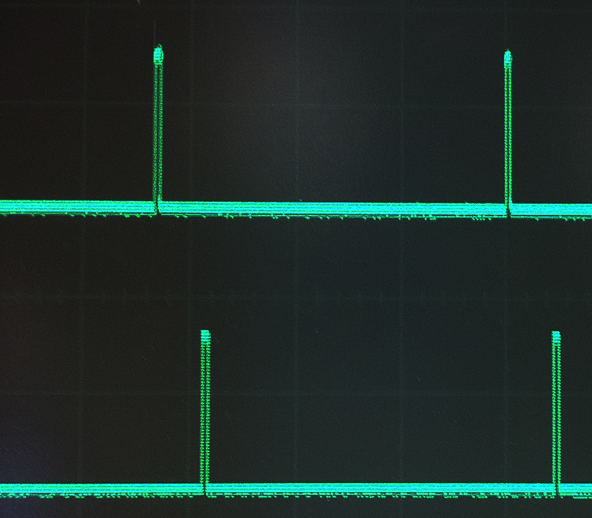
\includegraphics[width=0.24\textwidth]{include/unsync-scope}
		\label{fig:stereo-sync-hard1}
	}
	\subfloat[Synchronized \texttt{VSYNC}]{
		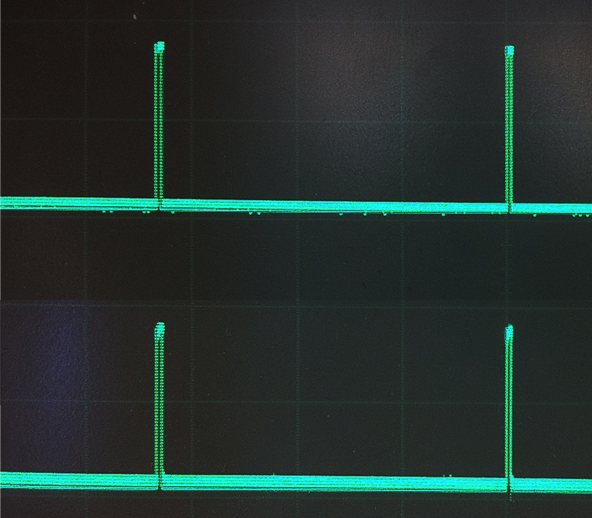
\includegraphics[width=0.24\textwidth]{include/sync-scope}
		\label{fig:stereo-sync-hard2}
	}
	\subfloat[Unsynchronized Frames]{
		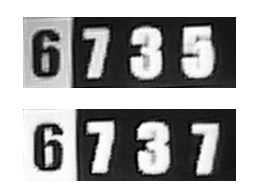
\includegraphics[width=0.24\textwidth]{include/unsync-img}
		\label{fig:stereo-sync-soft1}
	}
	\subfloat[Synchronized Frames]{
		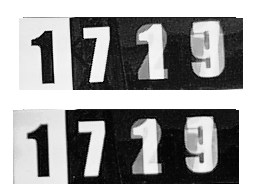
\includegraphics[width=0.24\textwidth]{include/sync-img}
		\label{fig:stereo-sync-soft2}
	}
	\caption{
		Verification of hardware and software camera synchronization for two
		Playstation Eye cameras. Note how only the synchronized cameras share a
		common \texttt{VSYNC} clock and capture identical readings of a
		millisecond resolution timer.
	}
	\label{fig:stereo-sync}
\end{figure*}

Hardware synchronization was achieved by  shorting the frame clock
(\texttt{VSYNC}) of the ``master'' camera to the frame trigger inputs
(\texttt{FSIN}) of the ``slave'' cameras. For electrical safety, each of the
cameras' USB grounds were shorted to force a common ground. This
synchronization guarantees that the cameras capture images simultaneously, but
does not guarantee that the images will be synchronized after the USB transfers
to the computers. Making direct use of the Video4Linux kernel module, software
synchronization was achived by fuzzy-matching of the the USB transfer
timestamps\footnote{\texttt{https://github.com/mkoval/stereo\_webcam}}.
Synchronization was verified in hardware by probing each camera's
\texttt{VSYNC} pin with an osilloscope (Figures ~\ref{fig:stereo-sync-hard1}
and ~\ref{fig:stereo-sync-hard2}) and and in software by recording images of a
millisecond-resolution timer (Figures ~\ref{fig:stereo-sync-soft1} and
~\ref{fig:stereo-sync-soft2}).

% 3. Baseline multiplexing using three cameras
% FIGURE: Effect of baseline on dead zone and maximum range.
% FIGURE: Graph of distance vs. disparity for both baselines.
\subsection{Baseline Multiplexing}
\label{sec:stereo-mux}
While unknown changes in the system's baseline is disasterous, having control
over the stereo camera's baseline can be extremely beneficial. Selecting the
best baseline is a balance of two opposing, but equally important, factors:
dead-zone and range. Decreasing the baseline shrinks the both the size of the
deadzone and the maximum range at which distances can be distinguished. This
maximum range exists because disparity is measured in pixels: there is no
discernable difference between any disparity less than one pixel. Multiplexing
between a 10 cm baseline (the \textit{narrow stereo}) and a 20 cm baseline (the
\textit{wide stereo}) combines the benefits of both baselines.

\begin{figure}
	\subimport{include/}{dist-disparity}
	\caption{
		Relationship between real-world distance and image disparity for
		10 cm and 20 cm baselines. Note that the 20 cm baseline has a maximum
		range approximately twice that of the 10 cm baseline.
	}
	\label{fig:stereo-dist-disparity}
\end{figure}

For a stereo camera, the relationship between distance and disparity can be
shown to be
\begin{equation*}
	x = \frac{bf}{n\sigma}
\end{equation*}
where $b$ is the baseline, $f$ is the camera's focal distance, and $\sigma$ is
the size of a pixel on the image sensor. By substituting the intrinsics
parameters of the Playstation Eye camera\footnote{$f = 3.15$ mm, $\sigma = 6$
$\mu$m} and setting $n = 1$ pixel, the maximum range of both baselines can be
evaluated. As can be seen in Figure ~\ref{fig:stereo-dist-disparity}, the 10 cm
and 20 cm baselines have theoretical maximum ranges of 5 m and 10 m
respectively. With the width of the course fixed at approximately 6 m, a
maximum range of 10 m is more than sufficient for navigation purposes.

% 5. Point correspondances: SSD BM on the CPU or SAD BM on the GPU?
\subsection{Reconstruction Algorithm}
\label{sec:stereo-correspond}
Due to the use of ROS as the basis for the Navigator's software architecture
(Section ~\ref{sec:robot}), the actual stereo reconstruction is done using the
standard \texttt{stereo\_image\_proc} ROS node. This node implements real-time
calibrated stereo by rectifying the images, applying a series of
texture-enhancing filters, and using a highly optimized sum-of-squared
difference (SSD) block-matching algorithm to point correspondences. This
disparity map is then converted into a three-dimensional point cloud in the
cameras' coordinate frame using the calibration parameters.

% 6. Software integration and cost map generation

\section{Lane Tracking}
\label{sec:lane}
% 1. Problems with other teams' approaches
% 2. Color space transformation, ground plane assumption
% 3. Creating and using a matched pulse-width filter (!)
% 4. Non-maximal supression (!)
% 5. Model fitting?
% 6. Lane width inference?
% 2. Creating and using a matched pulse-width filter (!)
\subsection{Matched Pulse-Width Filter}
Because the lines on the course are known to be uniformly three inches wide, an
obvious approach for isolating them from other objects is to use a digital
\textit{pulse-width filter} that is of the same width. Unfortunately, the
effects of perspective projection mean that the apparent width of lines in the
image depend upon their distance from the camera. To obtain useful output, such
a filter must be properly \textit{matched} to expected width of the line at
each point in the image.

Calculating this width requires knowledge of the three-dimensional point
corresponding to each pixel in the image. Assuming that the ground plane is
known and is parameterized by point $P$ and normal $n$, the three-dimensional
point $P$ that corresponds to pixel $p$ satisifes both
\begin{align*}
	(P - P_0) \cdot n     &= 0 \\
	\lambda M^{-1}_{int} p - P &= 0,
\end{align*}
where $M_{int}$ is the camera's intrinsic matrix and $\lambda$ is an arbitrary
constant.

Solving for $\lambda$ results in a closed-form expression containing
only known parameters. Substituting this value into the equation of the
line yields an intersection point of
\begin{equation*}
 	P = \left(\frac{n \cdot P_0}{n \cdot M^{-1}_{int} p}\right) M^{-1}_{int} p.
	\label{eq:line-point}
\end{equation*}
Using the new-found knowledge of point $P$, the pixel-width of the pulse-width
filter matched to pixel $p$ can easily be computed as
\begin{equation*}
	w = ||M_{int} P - M_{int} (P + W)||_2
\end{equation*}
where $W$ is a vector in direction $\langle 1, 0 \rangle$ of the same width as
the line and $|| \cdot ||_2$ denotes the Euclidean norm. Note that this is not
equivalent to $||W||_2$ because of the division implicit in the use of
homogeneous coordinates.

Once the expected width of the line at a given pixel is determined, seperate
horizontal and vertical pulse-width filters are created. Each of these filters
consists of a positive \textit{pulse} of width $w$ surrounded on both sides by
negative \textit{supports} of width $\frac{w}{2}$, normalized to have a zero
sum. When implemented, a rectified input image was used to guarantee that depth
does not vary within a row of pixels. This allows one filter to be pre-computed
per row, dramatically improving the algorithm's practical performance.

% FIGURE: Graph of the pulse-width filter.
% FIGURE: Output of the pulse-width filter.

% 3. Non-maximal Supression
\subsection{Non-Maximal Suppresion}
\label{sec:line-nonmax}
The matched pulse-width filter is extremely effective at isolating the line in
the image, but does not produce a clean enough output to be directly used for
model-fitting. In particular, the nature of digital filters guarantees that
there will be weak, spurious responses near true positives.

Inspired by Canny edge detection, non-maximal supression is an effective and
computationally efficient way of reducing such a response to a single point.
Considering the rows of the horizontally filtered image and the columns of the
vertically filtered image, a pixel is considered a maximum if and only if it
has a higher filter response than both of its neighbors. The maxima are then
thresholded to discard those that do not exhibit a sufficiently strong filter
response. This threshold was tuned to favor false positives and was set to
approximately 15\% of the filter's maximum response.

% TODO: Output of non-maximal suppression.
\section{Conclusion}
\label{sec:conclusion}
% ???

\section{Future Work}
\label{sec:future}
% 1. Further analysis of GPU-accelerated stereo
% 2. Stereo and/or IMU-based ground plane detection
% 4. Use stereo depth information to mask line false positives
% 3. Basic object recognition for flags, potholes, and road obstacles
% 4. Extensive testing in a software simulation (Gazebo)

\section{Acknowledgements}
% TODO: Make this phrasing less awkward.
I would like to thank all members of the Rutgers University IEEE Student Branch
for contributing to and supporting the Navigator. In particular, I am grateful
for Professor Predrag Spasojevic for serving as our faculty advisor and Adam
Stambler, Peter Vasilnak, Cody Schafer, Elie Rosen, Phillip Quiza, and Nitish
Thatte. This project would not be possible without support from our sponsors:
Knotts Corporation, 80/20 Inc., Optima Batteries, Github, and IEEE Region 1.
This project would also not be possible without the assistance provided by
Professor Kristin Dana, Steve Orbine, and John Scafidi of the Department of
Electrical and Computer Engineering and Joe Lippencott with the Department of
Industiral and Systems Engineering.

\end{document}
